\documentclass[14pt,a4paper]{article}
\usepackage[latin1]{inputenc}
\usepackage[T1]{fontenc}
\usepackage[english]{babel}
\usepackage{amsmath}
\usepackage{amsfonts}
\usepackage{amssymb}
\usepackage{makeidx}
\usepackage{amsthm}
\usepackage[margin=48pt]{geometry}
\usepackage[linesnumbered,ruled]{algorithm2e}
\usepackage{tikz}
\usetikzlibrary{automata, positioning}
\usepackage{float}

\def\code#1{\texttt{#1}}
\newtheorem{theorem}{Theorem}
\def\iff{\Leftrightarrow}
\theoremstyle{definition}
\newtheorem{madef}{Definition}
\newtheorem{prop}{Proposition}


\oddsidemargin  0in
\evensidemargin  0in
\textwidth   6.3in
\textheight  9.5in
\topmargin  -0.7in



\usepackage{fancyhdr}
\pagestyle{fancy}
\lfoot{Charles DUFOUR}
\rfoot{\today}



\author{Charles Dufour}
\title{Bachelor Project : \\
Reinforcement learning and robot navigation}
\begin{document}

\begin{titlepage}
\newcommand{\HRule}{\rule{\linewidth}{0.5mm}} % Defines a new command for the horizontal lines, change thickness here

\center % Center everything on the page
 
%----------------------------------------------------------------------------------------
%   HEADING SECTIONS
%----------------------------------------------------------------------------------------

\vspace{3cm}
\textsc{\LARGE \'Ecole polytechnique f\'ed\'erale de Lausanne}\\[0.5cm] % Name of your university/college
\textsc{\large Disopt}\\[1.5cm] % Name of your university/college
\textsc{\LARGE Semester project}\\[0.5cm] % Major heading such as course name
\textsc{\large }\\[0.5cm] % Minor heading such as course title

%----------------------------------------------------------------------------------------
%   TITLE SECTION
%----------------------------------------------------------------------------------------

\HRule \\[0.4cm]
{ \huge \bfseries Reinforcement learning and robot navigation}\\[0.4cm] % Title of your document
\HRule \\[1.5cm]
 
%----------------------------------------------------------------------------------------
%   AUTHOR SECTION
%----------------------------------------------------------------------------------------

\begin{minipage}{0.4\textwidth}
\begin{flushleft} \large
\emph{Student:}\\
Charles Dufour
\end{flushleft}
\end{minipage}
~
\begin{minipage}{0.4\textwidth}
\begin{flushright} \large
\emph{Supervisors:} \\
Jonas Racine\\% Supervisor's Name
Prof. Friedrich Eisenbrand 
\end{flushright}
\end{minipage}\\[5cm]

%----------------------------------------------------------------------------------------
%   LOGO SECTION
%----------------------------------------------------------------------------------------

% \includegraphics[width=0.5\linewidth]{Logo}\\[1cm] % Include a department/university logo - this will require the graphicx package
 
%----------------------------------------------------------------------------------------

\vfill % Fill the rest of the page with whitespace

\end{titlepage}



%\begin{titlepage}
%   \vspace*{\stretch{1.0}}
%   \begin{center}
%      \Large\textbf{Reinforcement learning and robot navigation}\\
%      
%      \large\textbf{ }\\
%      \large\textit{Bachelor Project}
%   \end{center}
%   \vspace*{\stretch{2.0}}
%   
%   \vfill 
%   {\centering Charles Dufour, EPFL\par}
%\end{titlepage}

\newpage

\tableofcontents

\newpage
\section{Theory}
\subsection{Introduction}


\emph{Reinforcement learning}\\
Reinforcement learning is learning what to do, how to map situations to actions so as to maximize
a numerical reward signal. The learner is not told which actions to take, but instead must discover
which actions yield the most reward by trying them. \cite{Sutton}

Some technical terms : 
\begin{itemize}
\item \emph{policy} : it is a mapping from the states to the actions
\item \emph{reward} : what our learning agent is trying to maximize
\item \emph{model} of the environment : the laws governing the environment 
\end{itemize}

"Reinforcement learning methods specify how the agent's policy is changed as a result of its experience"\cite{Sutton}



The usual way to formulate the reinforcement learning problem from a mathematical point of view is by using what we call Markov's decision processes (MDP's).

\subsection{MDP : Markov decision processes}



Markov's decision processes are composed by : 

\begin{itemize}
\item a set of states : $\mathcal{S}=\{s_0,s_1,\ldots\}$
\item a set of actions  : $A=\{a_1,a_2,\ldots \}$
\item a transition function :  $T(s,a,s') \sim  Pr(s'\mid a, s) \quad s,s' \in \mathcal{S}$ which gives the state transition probabilities
\item a reward function : $\mathcal{R}:\mathcal{S}\mapsto \mathbb{R} $
\item The Markov property : the transitions only depends on the current state and action
\end{itemize}


When an agent is learning in a MDP, what it observes is a sequence of states, actions and rewards: suppose the agent is in the state $s_0$ and chooses action $a_1$ and then end up in state $s_1$ with reward $r_1$; then the sequence observed is of the form : $s_0,a_1,s_1,r_1,s_2,\ldots$

Markov decisions processes are usually represented with graph : the nodes are the states and the directed edges from a node $Q$ are the actions an agent can choose to make while being in state $Q$, which will bring the agent in the state represented by the node at the endpoint of the edge as we can see in figure \ref{figure : graph_example}.


\begin{figure}[H]
\centering
    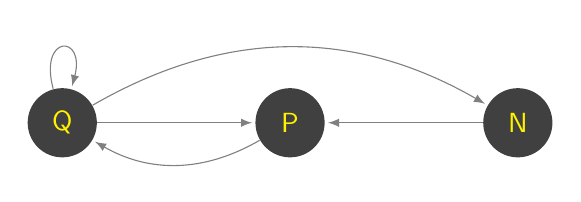
\begin{tikzpicture}[font=\sffamily]
    % Add the states
        \node[state,
              text=yellow,
              draw=none,
              fill=gray!50!black] (Q) {Q};
        \node[state,
              right=2cm of Q,
              text=yellow,
              draw=none, 
              fill=gray!50!black] (P) {P};
        \node[state,
              right=2cm of P,
              text=yellow,
              draw=none, 
              fill=gray!50!black] (N) {N};
              
                \draw[every loop,
        auto=right,
        >=latex,
        draw=gray,
        fill=gray]
        
        	(Q) edge[loop above](Q)
        	(Q) edge[bend left](N)
            (Q) edge[] (P)
            (P) edge[bend left] (Q)
            (N) edge[](P);
              
    \end{tikzpicture}
    \label{figure : graph_example}
        \caption{example of a graph representing a Markov Decision process}
\end{figure}  




\subsubsection{Policies and Value functions}

A policy : $\pi : \mathcal{S} \mapsto A $ is a mapping from states to action. If we follow this policy (way of behaving) we can define the value function for a policy in order to compare them, which links a state and its expected reward if we follow this policy.

The discount factor $\gamma $ helps making our learning agent more or less far-sighted : the greater $\gamma $ the more "impact" will have a late reward on our reward sequence, hence making the agent more conscious about these actions.

We define the return as : $G_t= R_{t+1}+\gamma R_{t+2}+ \dots = \sum_{k=0}^{\infty}\gamma^{k}R_{t+k+1} $

And $\pi(a\mid s) $ is the probability that $A_t=a$ if $S_t=s$

Then we can define the value of taking action $a$ in state $s$ while following the policy $\pi$ 

\begin{equation}
\begin{split}
q_{\pi}(s,a)&= \mathbb{E}[G_t\mid S_t=s, A_t=a]
\\&=\mathbb{E}[\sum_{k=0}^{\infty}\gamma^{k}R_{t+k+1}\mid S_t=s,A_t=a]
\\&= \sum_{r,s'}p(s',r\mid s,a)[r+\gamma v_{\pi}(s')]
\end{split}
\label{q(s,a)}
\end{equation}


And the value of a state s under a policy:
\begin{equation}
\begin{split}
v_{\pi}(s)&= \mathbb{E}[G_t \mid S_t=s]
\\&= \mathbb{E}[ \sum_{k=0}^{\infty}\gamma^t R_{t+k+1} \mid S_t = s ]
\\& =\sum_{a}\pi(a\mid s)\sum_{r,s'}p(s',r\mid s,a)[r+\gamma v_{\pi}(s')]
\end{split}
\label{v(s)}
\end{equation}

\subsubsection{Optimal policies and Optimal value function}

For finite MDP's, the value function can define a partial order in the space of policies : 
$$ 
\pi\leq \pi' \iff \pi (s)\leq \pi' (s) \quad \forall s \in \mathcal{S}
$$

An optimal policy is a policy which is greater or equal than any other policy. This is what we are interested to find.

\paragraph{Bellman optimality equations}

The optimal policy $\pi^*$ has  optimal value functions : $v_* $ and $ q_*$, which satisfy the relations below : 

\begin{equation}
v_{*}(s)=\max_{a} \sum_{s',r}p(s',r\mid s,a)[r+\gamma v_{*}(s')]
\label{bellman_opt_v}
\end{equation}

\begin{equation}
q_{*}(s,a)= \sum_{s',r}p(s',r \mid s,a)[r+\gamma \max_{a'}q_{*}(s',a')]
\label{bellman_opt_q}
\end{equation}

These are called the \emph{Bellman optimality equations}.


For finite MDP's these equations have a unique solution. We can note that if we know $v_{*}$ or $q_{*}$ a greedy approach to define a policy (best in the short term) becomes a long-term optimal solution : indeed defining a policy being greedy in function of $v_*$ implies that you go to the best state possible, the one with the bigger expected reward.


\subsection{Solving MDP's with dynamic programming}

In general we don't have all the information we need to compute the exact value of $v_{*}$ or even if we have them, we don't have the computational 
power needed. We often use approximation of value-function instead.


From now on we assume our MDP's are finite, even if it is possible to extend everything to infinite MDP's if we are careful enough to avoid the problematic ones.

\subsubsection{Policy iteration}

This method uses two processes : the first one is policy evaluation : we compute the value function of a policy for all the states $s \in \mathcal{S} $; then we use policy improvement to get a better policy by acting greedy.
\paragraph{Policy evaluation} 


We begin by setting arbitrary $v(s) \quad \forall s \in \mathcal{S}$.
Then we update using one of the following update rules : 

\begin{itemize}
\item $v_k(s)=\sum_{a \in A}\pi(a \mid s)\sum_{s',r}p(s',r\mid s,a)(r+\gamma v_k(s'))$ \quad this is called "iterative policy evaluation".
\item we can use the same update rule as before, but use new information as soon as it is available : this kind of upgrade algorithm are called in places.
\end{itemize}

From this we derive the algorithm \ref{algo1}.


\begin{algorithm}
\label{algo1}
    \SetKwInOut{Input}{Input}
    \SetKwInOut{Output}{Output}

    %\underline{function Euclid} $(a,b)$\;
    \Input{policy to evaluate $\pi$}
    \Output{$V \approx v_{\pi}$}
    Initialize $V = 0$\\
    \While{$\Delta \geq \epsilon$}{
    	$\Delta = 0$\\
    	\For{$s\in \mathcal{S}$}{
    	 $v=V(s)$\\
    	 $V(s)=\sum_{a}\pi(a\mid s)\sum_{s',r}p(s',r\mid a,s)[r+\gamma V(s')]$\\
    	 $\Delta = \max(\Delta,\mid v-V(s)\mid)$\\
    	 }
       	}
       	\Return{$V \approx v_{\pi}$}
    
    \caption{Iterative policy evaluation (in place)}
\end{algorithm}



\paragraph{Policy improvement}

Then we try to find a better policy : we try to determine whether we should change $\pi(s) $ to $ a\neq\pi(s)$. In order to do so, we try to first select action $a$ while being in state $s$ and then following the policy. If the expected reward we get by doing this choice is better than the one we get by simply following our policy, we should improve.

Mathematically speaking we will compare the value of taking action $a$ while being in the state s : $q_{\pi}(s,a)$ to the value of $s$: $v_{\pi}(s)$. Then we would greedily improve our policy this way.

The greedy update rule we use to improve our policy is from which we derive algorithm \ref{algo2} : 

$$ 
\pi'(s)=\text{arg}\max_{a \in A}q_{\pi}(s,a)
$$

\begin{algorithm}
\label{algo2}
    \SetKwInOut{Input}{Input}
    \SetKwInOut{Output}{Output}

    %\underline{function Euclid} $(a,b)$\;
    \Input{policy to improve $\pi$}
    \Output{$\pi'$ s.t : $\pi' \geq \pi$ }
    \For{$s\in \mathcal{S}$}{
    	$\pi'(s)=\text{arg}\max_{a \in A}q_{\pi}(s,a)$
    	}
       	\Return{$\pi'$}
    
    \caption{Policy improvement}
\end{algorithm}



\paragraph{Policy Iteration} By combining the two processes described before, we can derive an algorithm to sweep through all our states and upgrade our policy until the changes between each sweep is too small : it is controlled by a parameter $\epsilon$ and a parameter $\gamma$ (which we talked about previously).This is the algorithm \ref{algo3}.



The reason why the algorithm~\ref{algo3} works is called the the \emph{policy improvement theorem}:

\begin{theorem}
Let $\pi$ and $\pi'$ be any pair of policies such that  $\forall s \in \mathcal{S} : $
\begin{equation}
q_{\pi}(s,\pi(s))\geq v_{\pi'}(s) \label{th1}
\end{equation}
then :
\begin{equation}
\pi \geq \pi' \label{th2}
\end{equation}


Moreover if there is a strict inequality in all the states in \ref{th1} then there must be at least a strict inequality for one state in \ref{th2}
\end{theorem}


\begin{proof}
The idea of the proof is to expand the $q_{\pi}$ side until we get $v_{\pi'}(s)$ using Equation~\ref{q(s,a)} in page \pageref{q(s,a)}.

Indeed we have : 
\begin{equation}
\begin{split}
v_{\pi}(s) &\leq q_{\pi}(s,\pi'(s))
\\&=\mathbb{E}[R_{t+1}+\gamma v_{\pi}(S_{t+1})\mid S_{t}=s, A_{t}=\pi'(a)]
\\&=\mathbb{E}_{\pi'}[R_{t+1}+\gamma v_{\pi}(S_{t+1})\mid S_{t}=s]
\\& \leq \mathbb{E}_{\pi'}[R_{t+1}+\gamma q_{\pi}(S_{t+1},\pi'(S_{t+1}) \mid S_{t}=s]
\\& = \mathbb{E}_{\pi'}[R_{t+1}+\gamma \mathbb{E}_{\pi'}[R_{t+2}+\gamma v_{\pi}(S_{t+2})]\mid S_{t}=s]
\\& = \mathbb{E}_{\pi'}[R_{t+1}+\gamma R_{t+2}+\gamma^2 v_{\pi}(S_{t+2})\mid S_{t}=s]
\\& \leq \ldots
\\&= v_{\pi'}(s)
\end{split}
\end{equation}
\end{proof}


\begin{algorithm}
	\SetKwInOut{Input}{Input}
    \SetKwInOut{Output}{Output}
    
	\Input{arbitrary policy, stopping criterion $\epsilon$}
	\Output{estimation of the optimal policy and of its value function}
	
	Policy evaluation :\\
	    \While{$\Delta \geq \epsilon$}{
    	$\Delta = 0$\\
    	\For{$s\in \mathcal{S}$}{
    	 $v=V(s)$\\
    	 $V(s)=\sum_{a}\pi(a\mid s)\sum_{s',r}p(s',r\mid a,s)[r+\gamma V(s')]$\\
    	 $\Delta = \max(\Delta,\mid v-V(s)\mid)$\\
    	 }
       	}
     
     Policy improvement : \\
     policy-stable = true \\
     \For{$s \in \mathcal{S}$}{
     old-action= $\pi(s)$\\     
     $\pi(s)=\text{arg}\max_{a \in A}q_{\pi}(s,a)$\\
     \If{old-action $\neq \pi(s)$}{
     policy-stable = false}
     }
     \eIf{policy-stable}{
     \Return{$V \approx v^{*} \text{and} \quad \pi \approx \pi^{*}$}
     }{Go to Policy evaluation}
     
	\caption{Policy Iteration}
	\label{algo3}
\end{algorithm}

\subsubsection{Value Iteration}
Value iteration is another way of approximating an optimal policy : it combines in each of its sweep improvement and evaluation in algorithm \ref{algo4}.

\begin{algorithm}
	\SetKwInOut{Input}{Input}
    \SetKwInOut{Output}{Output}
    \label{algo4}
    
    \Input{policy}
    \Output{estimate of optimal policy}    
	    
    Initialize V arbitrarily 
    \While{$\Delta \geq \epsilon$}{
    	$v=V(s)$\\
    	$V(s)=\max_{a}\sum_{s',r}p(s',r\mid s,a)[r+\gamma v_{k}(s')]$\\
    	$\Delta =\max(\Delta,\mid v-V(s) \mid)$\\    	
    }
    \Return{$\pi \approx \pi^{*}$ s.t : $\pi(s)=\text{arg}\max_{a}\sum_{s',r}p(s',r\mid s,a)[r+\gamma v_{k}(s')]$}
    

    
\caption{Value iteration}
\end{algorithm}


Here the main difference is the $\max$ in the evaluation line.


\subsubsection{Other types of DP method}

There exists some others dynamic programming algorithm to solve these problems : 
\begin{itemize}
\item Asynchronous Dynamic programming : it doe not sweep amongst all the states at each iteration. They are in place iterative DP algorithms.
\item General Policy Iteration (GPI): they are mixing the two components of policy iteration (evaluation and improvement) a little bit more than the algorithm we already saw.
\end{itemize}


\subsubsection{Efficiency of the DP method}


\newpage

\section{Journal}
\begin{description}
\item[28.02.2018] finished reading chapter 2 Sutton's book about the \code{k-bandits problem} : implementation of simple algorithms of the book on jupyter notebook in \code{Rl-sandbox}
\item[01.03.2018] initiated the Latex journal 
\item[04.03.2108]read the notebook about \code{numpy} and tried to go on with the lecture of the literature--> have to read again the example about the golf 

finished the chapter 3 
\item[12.03.2018] read chapter three again and made a summary of it

Then tried to attack the street racer problem 

\item[15.03.2018] tried to understand exactly what the problem of the street racing was about and tried to define a real reward function after coding the matrices for each action
Then went back to studying chapter 4 in order to implement the policy evaluation/improvement functions 

\item[16.03.2018] finished reading chapter 4 of Sutton's book continued the summary
\item[17.03.2018] finished typing the r\'{e}sum\'{e} so that I could concentrate on the actual code. I'm not sure about including a subsubsection about the efficiency of the DP method but for now I'm just putting the title to remember .

I have a little problem of references for my first graph but I'll see to that later 

\begin{equation}
v_{\pi}(s)=R(s)+\gamma \sum_{s \in \mathcal{S}} P(s' \mid s,\pi(s))v_{\pi}(s')
\label{bellman1}
\end{equation}

Et je pense que cette equation traduit  bien le cas non stochastic, est-ce que j'explique en plus ?

Then I tried to finish the street racing program but too many bugs appeared so I stop for today, and I'll try again tomorrow

\item[21.03.2018] Finished design the matrices and the model for the racing car, but issues seem to appear , the algorithm doesn't seem to work

\item[22.03.2018] fixed issues in the code : still strange things happening : the score get optimum too quickly....

\end{description}


\newpage

\bibliographystyle{plain}
\bibliography{ref}
\addcontentsline{toc}{section}{References}


\end{document}


%\paragraph{The Bellman equation}
%\begin{equation}
%v_{\pi}(s)=R(s)+\gamma \sum_{s \in \mathcal{S}} P(s' \mid s,\pi(s))v_{\pi}(s')
%\label{bellman1}
%\end{equation}
%
%\begin{equation}
%v_{\pi}(s)=\sum_{a}\pi(a\mid s)\sum_{s',r}p(s',r \mid s,a)[r+\gamma v_{\pi}(s')]
%\label{bellman2}
%\end{equation}
%
%These are two formulations of the bellman equation used to compute optimal policies by iteration : \eqref{bellman1} is from the MOOC and \eqref{bellman2} is from Sutton's book \cite{Sutton}